% Stroke Amnesia: Why Language Models Still Need a Canvas
% Author: Poonam Nair
% Compiles with pdflatex. No proprietary class files required.

\documentclass[10pt,twocolumn]{article}

% ---- Packages ----
\usepackage[a4paper,margin=2cm]{geometry}
\usepackage[utf8]{inputenc}
\usepackage[T1]{fontenc}
\usepackage[activate={true,nocompatibility},final,kerning=true,spacing=true,factor=1100,stretch=10,shrink=10,expansion=false]{microtype}
\usepackage{graphicx}
\usepackage{xcolor}
\usepackage{tikz}
\usetikzlibrary{positioning,arrows.meta,fit,backgrounds}
\usepackage{amsmath,amssymb}
\usepackage{booktabs}
\usepackage{enumitem}
\usepackage{caption}
\usepackage{listings}

% Define JavaScript language for listings
\lstdefinelanguage{JavaScript}{
  keywords={break, case, catch, const, continue, debugger, default, delete, do, else, false, finally, for, function, if, in, instanceof, let, new, null, return, switch, this, throw, true, try, typeof, var, void, while, with},
  morecomment=[l]{//},
  morecomment=[s]{/*}{*/},
  morestring=[b]',
  morestring=[b]",
  sensitive=true,
}

% Code listing style
\definecolor{codebg}{HTML}{F6F4EF}
\definecolor{codecomment}{HTML}{6A6A6A}
\definecolor{codekw}{HTML}{1F4E79}
\definecolor{codestr}{HTML}{8B4513}
\lstdefinestyle{paperjs}{
  backgroundcolor=\color{codebg},
  basicstyle=\ttfamily\scriptsize,
  commentstyle=\color{codecomment}\itshape,
  keywordstyle=\color{codekw}\bfseries,
  stringstyle=\color{codestr},
  language=JavaScript,
  breaklines=true,
  breakatwhitespace=true,
  showstringspaces=false,
  columns=fullflexible,
  keepspaces=true,
  framesep=4pt,
  framerule=0pt,
  xleftmargin=4pt,
  xrightmargin=4pt,
  aboveskip=8pt,
  belowskip=4pt,
}
\usepackage{hyperref}
\usepackage{authblk}
\usepackage{titlesec}
\usepackage{abstract}

% ---- Style tweaks ----
\hypersetup{
  colorlinks=true,
  linkcolor=black!70,
  citecolor=black!70,
  urlcolor=black!70,
}
\titleformat*{\section}{\normalsize\bfseries}
\titleformat*{\subsection}{\normalsize\bfseries\itshape}
\setlength{\columnsep}{0.7cm}
\renewcommand{\abstractname}{\normalsize\bfseries Abstract}
\setlength{\absleftindent}{0pt}
\setlength{\absrightindent}{0pt}

% ---- Custom commands ----
\newcommand{\term}[1]{\textit{#1}}
\newcommand{\inky}{\textsc{Inky}}

% ---- Title ----
\title{\Large\bfseries Stroke Amnesia:\\
Why Language Models Still Need a Canvas}

\author[1]{Poonam Nair\thanks{Correspondence: \href{mailto:poonnair@gmail.com}{poonnair@gmail.com}. Melbourne, Australia.}}
\affil[1]{Independent}

\date{May 2026}

\begin{document}
\twocolumn[
  \begin{@twocolumnfalse}
    \maketitle
    \begin{abstract}
      \noindent
      Large language models can describe drawings fluently and emit
      SVG, Canvas, or TikZ code that renders to recognisable images.
      We argue these abilities do not constitute robust drawing
      competence. \inky{} is a coding-agent-driven canvas animation
      pipeline that turns user-provided storyboard references into
      hand-drawn, code-rendered 2D animations. The system is a
      scaffolding and rendering harness rather than a fixed set of
      examples: each project defines its own canvas dimensions,
      frame count, and a scaffold of intermediate artifacts
      including requirements, construction blueprints, in-between
      plans, and renderer stubs. Through this generic pipeline, we
      observe consistent failure patterns --- \term{stroke amnesia},
      \term{compositional collapse}, and \term{patch reflex} ---
      and show how externalised structure, visual feedback, and
      root-cause redraw rules push outputs back toward coherence.
      We argue that the missing capability is not pixel synthesis
      but a durable latent canvas that tracks object identity, part
      ownership, and contact across generation and revision. We
      close with an evaluation agenda that grades \emph{process,
      structure, and repair behaviour}, independent of final image
      content, and three benchmark tasks designed to discriminate
      models on these axes.

      \medskip
      \noindent\textbf{Keywords:} large language models, drawing,
      multimodal evaluation, agentic systems, generative art,
      benchmarks.
    \end{abstract}
    \vspace{1em}
  \end{@twocolumnfalse}
]

% =====================================================================
\section{Introduction}
% =====================================================================

A model that can describe a hand is not yet a model that can keep the
wrist attached. This paper is a position statement on a gap that has
become visible only recently, as multimodal models, tool use, and
agentic coding loops have made it plausible for language models to
act through canvases, SVG, browsers, and visual feedback. They can now
\emph{try, inspect, and revise}. We argue that this revision loop is
where the gap appears most sharply: models can write code that
produces drawings, and they can describe what is wrong with the
result, but they cannot reliably repair the result without external
structure.

The argument is grounded in \inky{}, a coding-agent-driven canvas
animation pipeline that turns user-provided storyboard references
into hand-drawn, code-rendered, inspectable 2D animations. \inky{}
is not a research artefact and not a fixed showcase; it is a
scaffolding and rendering harness. Given a storyboard, it creates
a project folder, generates intermediate artifacts (requirements,
construction blueprints, in-between plans, renderer stubs), and
hands a coding agent a structured workspace to fill in. The
project's canvas dimensions, frame count, and material kit are
defined per project rather than fixed by the system. Its design
rules, accumulated across many user projects, document the
failure modes that matter in practice: floating limbs,
disconnected clothing, mistaken speech-bubble ownership, guide
marks promoted to final objects, and texture used to hide unclear
construction. We treat these rules as evidence.

We make three contributions.

\begin{enumerate}[leftmargin=*,nosep,itemsep=0.25em]
  \item A failure taxonomy for LLM-mediated drawing, grounded in a
    production pipeline rather than synthetic prompts, including
    three named phenomena: \term{stroke amnesia}, \term{compositional
    collapse}, and \term{patch reflex}.
  \item An engineering pattern for storyboard-to-canvas animation
    using explicit intermediate artifacts (requirements,
    lighthouses, construction blueprints, semantic review boards,
    visual diffs) that survives model swaps.
  \item A benchmark agenda that grades drawing as a process --- with
    decomposed scoring across recognisability, spatial relation,
    part attachment, text readability, repair quality, and
    continuity --- and three concrete tasks designed to be hard for
    today's models in informative ways.
\end{enumerate}

The paper is deliberately constructive. We critique the implicit
claim that LLMs ``can draw'' because they can emit Canvas or SVG
snippets, but the centre of gravity is the pipeline and the
benchmark, not the critique.

% =====================================================================
\section{Background and Scope}
% =====================================================================

\subsection{What we mean by ``drawing''}

In this paper, drawing is a \emph{process trace that places visual
marks on a 2D canvas so that objects, bodies, text, motion, and
material texture are readable without the source prompt}. In \inky{},
this includes storyboard redraws, comic frames, captions, speech
bubbles, hand-drawn texture, and frame-by-frame animation. We
explicitly exclude photorealistic text-to-image diffusion, 3D
modelling, music notation, handwriting as a separate recognition
problem, and claims about final production art quality. Our concern
is structural readability of 2D illustrative drawing produced through
code.

\subsection{What we mean by ``bad''}

We measure ``bad'' relative to two reference points: (i) the model's
own language competence on the same subject, and (ii) a competent
human sketcher working under similar time pressure. The failure is
not primarily aesthetic. It is structural: parts detach, proportions
drift, intended objects become blobs, and repairs are made with
patches rather than rebuilt geometry. A model that can write a
correct paragraph describing a person holding a mug can produce a
rendering in which the hand floats next to the cup.

\subsection{Why now}

Three shifts make this paper timely. First, multimodal models can now
see their own output, which makes the gap between description and
execution observable in a single conversation. Second, agentic coding
loops allow models to act, render, inspect, and revise --- the
ingredients of drawing as practice rather than synthesis. Third, the
external rendering stack (browser canvases, headless screenshots,
visual diff libraries) is now cheap enough to wire into a tight loop.
The bottleneck has moved from \emph{can the model emit drawing code?}
to \emph{can the model repair drawing structure when shown that it is
wrong?}

% =====================================================================
\section{The \inky{} Pipeline}
% =====================================================================

\subsection{System overview}

\inky{} renders 2D animations from user-provided storyboard
references using a coding agent (e.g.\ Claude or a similar
code-writing model) that operates over a structured repository of
design rules, skills, and project files. The runtime application
itself does not call a model API; the ``drawing brain'' is the
agent operating on the codebase. The user-facing artefact is a
browser preview with Play/Pause, timeline scrubbing, speed
control, PNG and MP4 export.

Canvas dimensions, frame count, frame rate, and material kit are
defined per project, not by the system. A typical project might
use a $960 \times 620$ canvas at 12\,FPS over roughly 96 frames,
but each parameter is configurable through the project's
\texttt{requirements.md} and renderer stub. The drawing primitive
is JavaScript Canvas: paths, ellipses, fills, text, material
strokes, procedural texture, and frame schedules. Helper
functions wrap these into material strokes, speech bubbles,
captions, body parts, props, and animated scenes.

\subsection{The end-to-end agent pipeline}

Given a storyboard image and a one-line user prompt (e.g.\
``animate a cat playing with yarn in ink and watercolour style''),
\inky{} expects the agent to work through a ten-step pipeline:
(1) create a new folder under \texttt{projects/<project-name>/}
(typically via \texttt{npm run storyboard:start});
(2) save the original storyboard in
\texttt{projects/<project-name>/image/}; (3) extract the
individual panels into \texttt{projects/<project-name>/%
storyboard/} (\texttt{npm run extract:storyboard});
(4) write \texttt{requirements.md} with the
requested style and structural notes; (5) generate construction
blueprints from the source panels (\texttt{npm run
storyboard:blueprint}); (6) redraw the scene in
canvas code using the storyboard as a lighthouse, not a tracing
source; (7) remove storyboard-only marks such as panel numbers,
borders, long guide arrows, and construction lines; (8) animate
between the panels with in-between frames (\texttt{npm run
storyboard:inbetween}); (9) run polish checks for body
connections, clothing clarity, props, speech bubbles, texture,
and flicker (\texttt{npm run storyboard:polish}, \texttt{npm run
storyboard:visual-diff}, \texttt{npm run storyboard:semantic});
and (10) verify the browser preview and export controls.

This end-to-end pipeline is distinct from the nine-step
\emph{drawing order} introduced later in \S\ref{sec:drawing-order};
the agent pipeline covers project creation, scaffolding, and
review, while the drawing order governs how a single frame is
constructed inside that scaffold.

\subsection{Why Canvas, not SVG or diffusion}

Canvas is deterministic, browser-native, easy to capture frame by
frame, and compatible with procedural brush systems. \inky{} avoids
pasting source images or relying on diffusion output because the
point is \emph{controllable construction and editable animation}. The
representation chosen is not a stylistic preference; it is a
commitment to a substrate where every mark has a code-level cause.

\subsection{The effective prompt}
\label{sec:effective-prompt}

The agent's effective prompt is not a single string. It is a set of
files: an \texttt{AGENTS.md} that defines obligations, material
tools, failure modes, and quality gates; a \texttt{DESIGN.md} that
defines aesthetic and structural rules; per-skill \texttt{SKILL.md}
files for specialised procedures (\texttt{storyboard-animation-%
pipeline}, \texttt{reference-lighthouse}, \texttt{frame-construction-%
planner}, \texttt{inbetween-frame-planner}, \texttt{semantic-clarity-%
auditor}, \texttt{frame-consistency-auditor}, \texttt{animation-%
polish-pass}, \texttt{caption-subtitle-tooling}, and
\texttt{comic-speech-bubble-tooling}); and a per-project
\texttt{requirements.md} that captures the brief. Context is
externalised into the filesystem, so the agent re-reads the relevant
artefact rather than carrying everything in prompt memory.

\subsection{Project structure}

Each render project occupies a fixed folder layout:

\begin{verbatim}
projects/<project-name>/
  image/       # original source image
  prompt/      # user directions, corrections
  storyboard/  # frames, requirements,
               # ledgers, blueprints,
               # in-between plans
  outputs/     # PNG frames, MP4, contact
               # sheets, exports
\end{verbatim}

\noindent
The structure is load-bearing rather than cosmetic: the agent is
instructed not to copy old experiments, scratch files, or unrelated
outputs into a new project folder, because cross-project contamination
is itself a documented failure mode.

The skill files under \texttt{skills/} follow the open Agent
Skills format (a folder per skill containing a \texttt{SKILL.md}
with YAML frontmatter and prose instructions, with optional
bundled resources). The format was originally developed by
Anthropic and adopted as an open standard; \inky{}'s skills are
portable in principle, not bespoke to one model provider.

\subsection{Repository layout}

For readers consulting the repository alongside this paper, the
mapping is straightforward. \texttt{AGENTS.md} and \texttt{DESIGN.md}
at the repository root define the load-bearing prompt material
discussed in \S\ref{sec:effective-prompt}. The
\texttt{skills/} folder contains the per-skill \texttt{SKILL.md}
files referenced throughout. The \texttt{src/} folder contains the
runtime: \texttt{material-tools.js} (brush kit and pressure
profiles), \texttt{rough-accent-tools.js} (guarded RoughJS),
\texttt{speech-bubble-tools.js} (bubble construction and
ownership validator), and \texttt{caption-tools.js}. Pipeline
scripts live under \texttt{tools/} as a series of Node \texttt{.mjs}
files, each surfaced as an \texttt{npm run storyboard:*} command
(scaffolding, blueprint generation, in-between planning, polish
pass, visual diff, semantic review, material preview).
Per-project artifacts accumulate under \texttt{projects/}.

\subsection{Material tools}

Rather than a single ``drawing'' API, \inky{} exposes a kit of
roughly two dozen named brush helpers in
\texttt{src/material-tools.js}. Each entry pairs a stroke
configuration (size, thinning, smoothing, jitter, alpha, hatch
length) with a pressure profile and a written \texttt{useWhen}
clause that tells the agent when the brush applies:
\texttt{technical-pen} for crisp outlines and prop edges,
\texttt{dip-ink} or \texttt{brush-pen} for expressive silhouettes
and hair, \texttt{ballpoint-pen} for scratchy doodles,
\texttt{marker} for translucent fills, \texttt{graphite-pencil}
and \texttt{colored-pencil} for construction and dry colour,
\texttt{wax-crayon} and \texttt{oil-crayon} for wax-gap texture,
\texttt{charcoal} for smoky shadow, \texttt{watercolor},
\texttt{ink-wash}, \texttt{salt-watercolor}, \texttt{gouache},
\texttt{acrylic}, and \texttt{oil-paint} for paint effects, and
\texttt{airbrush}, \texttt{sponge}, and \texttt{screen-tone} for
specific effects. Two auxiliary helpers do work that prompts
alone cannot reliably do: \texttt{ensureReadableColor()} adjusts
text-bearing shapes against varying backgrounds with a contrast
target and returns whether the colour had to be adjusted, and
\texttt{drawCoherentPaperGrain()} produces seeded paper tooth
that is stable across frames instead of random per-frame
speckle. The paper-grain function is itself a continuity
countermeasure: shimmer in locked backgrounds is one of the
visual-diff stage's named targets.

The kit acts as a soft DSL. It constrains the action space at
the exact point the model is most likely to drift --- choosing
``hand-drawn'' as a style word and emitting noisy texture rather
than committing to a medium with structural implications. The
kit is also defensive: the RoughJS accent helper exposes
explicit arrays \texttt{ROUGH\_SAFE\_USES} and
\texttt{ROUGH\_AVOID\_USES} in code, restricting it to non-
semantic accents (background texture, dust, sparkle, paper
edges) and excluding speech bubbles, readable text, labels,
borders, desks, frames, hands, faces, body silhouettes, and
story-critical contact points. The constraint is encoded as
data, not only as text in a prompt.

\subsection{Non-LLM components}

Several components in the loop are deterministic tools rather than
model calls: storyboard extraction, project scaffolding,
construction blueprint generation, in-between schedule generation,
speech-bubble and caption-track generation, frame rendering, visual
diffing, semantic review board generation, browser preview, and MP4
assembly. The runtime stack is Vite over vanilla HTML/CSS/JS with
Canvas 2D for drawing. Node scripts (one per pipeline stage) live
under \texttt{tools/}, each invoked through an \texttt{npm run
storyboard:*} command. Production dependencies are deliberately
small: \texttt{perfect-freehand} for pressure-aware stroke
generation, \texttt{chroma-js} for colour operations,
\texttt{simplex-noise} for seeded texture noise, \texttt{d3-ease}
for animation curves, \texttt{pixelmatch} and \texttt{pngjs} for
pixel-diff review, \texttt{roughjs} for guarded non-semantic
accents, \texttt{paper} as an optional vector-graphics layer,
\texttt{jszip} for project bundling, and \texttt{mp4-muxer} as a
deprecated MP4 path scheduled for replacement with Mediabunny.
ImageMagick is used as a system tool for contact-sheet composition
and is not an npm dependency.

\subsection{Quality gates}

Before final export, the pipeline requires the following checks:
source-as-lighthouse with anchors, contact points, and silhouettes
identified; every important body chain connected; clothing and limbs
forming plausible parent-child chains; recurring props visible when
the scene implies them; chosen brush kit supporting the look without
hiding unclear construction; storyboard-only guide marks absent from
the final canvas; a polish-pass run after the first render;
root-cause redraw rather than cover-up patches; in-between frames
inspected, not only key frames; visual-diff review for flicker,
locked-background drift, vanishing props, and bubble jumps; and
browser controls (Play, Pause, speed, scrub, PNG and MP4 export)
verified end-to-end. When captions or speech bubbles are present, CC
toggle, VTT/SRT export, text wrapping, tail ownership, and bubble
placement are checked explicitly.

\subsection{Pipeline stages}

Figure~\ref{fig:pipeline} summarises the stages. A drawing is not
``done'' when the agent emits final code; it is done when an
explicit review pass --- browser preview, visual diff, export check,
project-specific gates --- accepts the frame sequence. There is no
autonomous stop signal.

\begin{figure*}[t]
  \centering
  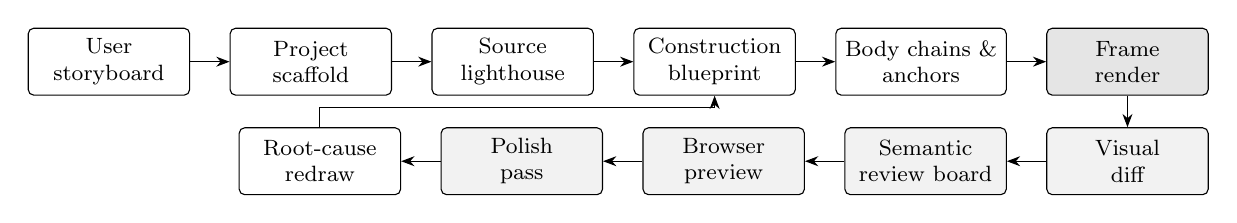
\begin{tikzpicture}[
      node distance=0.4cm and 0.5cm,
      box/.style={rectangle,draw,rounded corners=2pt,minimum height=0.85cm,minimum width=2.05cm,align=center,font=\footnotesize},
      review/.style={box,fill=black!5},
      art/.style={box,fill=black!10},
      ->,>=Stealth,
    ]
    \node[box] (story) {User\\storyboard};
    \node[box,right=of story] (scaffold) {Project\\scaffold};
    \node[box,right=of scaffold] (lh) {Source\\lighthouse};
    \node[box,right=of lh] (bp) {Construction\\blueprint};
    \node[box,right=of bp] (chain) {Body chains \&\\anchors};
    \node[art,right=of chain] (render) {Frame\\render};
    \node[review,below=of render] (diff) {Visual\\diff};
    \node[review,left=of diff] (semantic) {Semantic\\review board};
    \node[review,left=of semantic] (preview) {Browser\\preview};
    \node[review,left=of preview] (polish) {Polish\\pass};
    \node[box,left=of polish] (repair) {Root-cause\\redraw};
    \draw (story) -- (scaffold);
    \draw (scaffold) -- (lh);
    \draw (lh) -- (bp);
    \draw (bp) -- (chain);
    \draw (chain) -- (render);
    \draw (render) -- (diff);
    \draw (diff) -- (semantic);
    \draw (semantic) -- (preview);
    \draw (preview) -- (polish);
    \draw (polish) -- (repair);
    \draw (repair.north) |- ([yshift=-0.15cm]bp.south) -- (bp.south);
  \end{tikzpicture}
  \caption{The \inky{} pipeline, drawn generically: any user
    storyboard becomes a scaffolded project that flows through
    construction (top row, left to right) and review (bottom row,
    right to left). Failures discovered in review trigger
    \emph{root-cause redraw} from the construction blueprint, not
    patches over the rendered frame.}
  \label{fig:pipeline}
\end{figure*}

% =====================================================================
\section{Three Named Failure Modes}
% =====================================================================

Across many projects, three failure modes recur often enough to
deserve names. They are not mutually exclusive --- a single defective
frame often exhibits all three --- but naming them makes prompts,
review checklists, and benchmarks more precise.

\subsection{Stroke amnesia}

A model emits a stroke, then loses track of what the stroke meant.
Earlier marks become ambiguous to its own attention: a guide arrow
becomes a wire or a limb in the final rendering; a construction line
becomes a decorative element; a speech-bubble tail tracks the wrong
speaker. The repo guards against this with explicit instruction:
panel numbers, borders, labels, long arrows, long jump or throw arcs,
and construction lines must be removed or translated into actual
animation timing, never left on the final canvas. The fact that this
guard exists in writing is itself evidence: the agent reliably
promotes these marks to final objects when the instruction is absent.

The root cause is not a missing concept of ``arrow versus wire'';
the model can explain the difference. The cause is the lack of
durable ownership: there is no inspectable record stating that
\emph{this mark belongs to construction, not to the final scene}.

We call this \term{stroke amnesia}. The signature is that the model
will defend the offending mark when asked, because by the time it is
asked, the mark has been reabsorbed into ``what the drawing is.''

\subsection{Compositional collapse}

The model can draw a cat. It can draw a kettle. Asked to draw a cat
to the left of a kettle on a table, with the cat watching steam rise,
relations begin to fail: the cat sits on top of the kettle, the
kettle floats above the table, or the steam emerges from the cat.
Composition breaks when several relations must hold at once: a
character talks while holding papers, a bubble must avoid the face, a
prop must remain on the desk, and the same object must stay visible
across frames.

We call this \term{compositional collapse}: the rate at which
relational constraints are satisfied appears to fall non-linearly as
the number of simultaneous constraints rises. The phenomenon is
familiar from generative image models; what is new is that an
agentic loop with vision feedback does not, on its own, fix it.

\subsection{Patch reflex}

Shown a defect, the model often repairs the rendered output rather
than the underlying construction. The repo enumerates the specific
cover-ups it has had to forbid: cover-up shapes, eraser strokes,
white patches, opacity tricks, and decorative texture. Patches
succeed locally and fail under animation, when the camera moves, or
when the defect recurs across frames. A particular case worth naming
is the speech-bubble tail: the repo treats visible circles, ovals,
socket rings, and dot trails as bugs --- those marks belong only to
thought bubbles, and the speech-bubble body and tail must be
constructed as one continuous closed path, then filled and stroked
once.

We call this \term{patch reflex}. It is the drawing analogue of a
common failure in code generation: editing the symptom rather than
the cause. \inky{}'s most load-bearing rule is therefore not
stylistic but procedural --- the named \emph{Root-Cause Redraw Rule}:
when a rendered frame has a bug, fix the cause and rebuild the
affected shape or layer from its construction anchors using the
source lighthouse, requirements, and neighbouring frames, then
rerender. Cover-ups are not permitted.

\subsection{Why these three matter}

Stroke amnesia attacks identity. Compositional collapse attacks
relation. Patch reflex attacks repair. Each maps to a missing
capability rather than a missing skill. A larger model with no other
changes will likely improve planning and code syntax, but we expect
gains on these three axes to plateau without (i) durable
representations of object identity and (ii) training pressure on
repair behaviour, not only on final images.

% =====================================================================
\section{Workarounds in \inky{}}
% =====================================================================

\inky{}'s pipeline is, in effect, a catalogue of engineering
workarounds for the three failures above. We summarise the ones that
have proven most durable, with a note on which we believe survive
model swaps.

\subsection{Source lighthouse and construction anchors}

Before detailed rendering, the agent produces a \emph{source
lighthouse}: an interpretation of the storyboard reference that names
body chains, contact points, risky shapes, and storyboard-only
marks. These become construction anchors that subsequent stages must
respect. The lighthouse is explicitly not a copy of the source; it is
a structural reading of it. This single workaround produced the
largest practical quality jump we observed.

The lighthouse is also externalised as imagery, not only text. A
dedicated tool, \texttt{make-construction-blueprints.mjs}, takes
each source frame and uses ImageMagick to compose a board that
joins the full source on the left with a vertical strip of
semantic crops on the right (face, hands, action props). The
board is paired with a markdown file naming attachment chains,
risky shapes, the silhouette gate, and the detail-lock rule.
The agent therefore consults the lighthouse not as a paragraph
of text but as a rendered, croppable, inspectable artefact that
survives across sessions.

\subsection{Parent--child attachment chains}

A specific construction discipline does much of the work against
\term{compositional collapse}: every body and costume follows a
parent--child chain. Clothing is not floating decoration. Torso owns
the shirt hem; the shirt hem overlaps the waistband; the waistband
owns the leg openings; the leg openings own the legs. When the pose
shifts, bends, or rotates, the clothing anchor moves with the body
rather than as an independent shape. The repo enforces this with
explicit examples: if the source specifies ``shorts,'' the agent
must draw a waistband, two leg panels or openings, a centre seam or
crotch split, and legs exiting underneath. A single rounded blue
shape is logged as a clarity failure, not a stylistic choice. The
chain is the durable structure that survives re-rendering across
frames.

The rule is not only written; it is mechanised. In a typical
\inky{} renderer, the function \texttt{shortsGeometryForPose}
computes the waistband, leg edges, and openings from the torso
geometry, and \texttt{anchorLegChainsToShorts} re-anchors the leg
chains to those openings before any limb is drawn. The renderer
then uses \texttt{straightMaterialShape} --- not the smoothed
closed-path variant --- so the leg panels render as four-sided
shapes with a visible centre seam rather than a single rounded
blob. The structural rule and the structural code are the same
artefact:

\begin{lstlisting}[style=paperjs,label={lst:shorts},caption={Illustrative renderer pattern: the parent--child chain encoded in geometry rather than prompt text. Coordinates are derived from torso anchors and the panels render as straight-edged closed shapes.}]
const leftLeg = [
  [leftEdge, waistBottomY - 1],
  [centerX - 4, waistBottomY],
  [centerX - 5, legBottomY - 2],
  [leftEdge + 12, legBottomY + 3],
  [leftEdge - 5, waistBottomY + 20]];
const rightLeg = [
  [centerX + 4, waistBottomY],
  [rightEdge, waistBottomY - 1],
  [rightEdge + 5, waistBottomY + 20],
  [rightEdge - 12, legBottomY + 3],
  [centerX + 5, legBottomY - 2]];
const waistband = [
  [leftEdge - 4, waistTopY],
  [rightEdge + 4, waistTopY],
  [rightEdge + 2, waistBottomY],
  [leftEdge - 2, waistBottomY]];

straightMaterialShape(leftLeg,  /*...*/);
straightMaterialShape(rightLeg, /*...*/);
straightMaterialShape(waistband,/*...*/);

// centre seam
line([[centerX, waistBottomY],
      [centerX, legBottomY - 1]], 1.9, ...);
\end{lstlisting}

\noindent
Three points are worth surfacing. First, the openings are derived
from the torso, so a pose change automatically moves them. Second,
the legs are explicitly straight-edged closed paths rather than
ellipses or rounded blobs, which prevents the documented ``single
rounded blue shape'' failure mode at the geometry level. Third, the
centre seam is a separate \texttt{line()} call, not a decorative
afterthought --- it is constructed in the same step as the panels,
not patched in later.

\subsection{The nine-step drawing order}
\label{sec:drawing-order}

Decomposed layering is not a style preference; it is encoded as a
strict construction order with nine steps: (1) paper and chosen
material background, (2) simple construction anchors, (3) body
chains and prop contact points, (4) main silhouette, (5) removal
or translation of storyboard-only guide marks, (6) ink contours,
(7) dry colour, watercolour, gouache, pencil, crayon, charcoal, or
other chosen material texture, (8) dense hatching and texture, and
(9) a final clarity pass. The order matters because later stages
cannot modify foundational structure without revisiting earlier
ones, and because step 5 --- explicit removal of guide marks --- is
the structural countermeasure to \term{stroke amnesia}.

The transition between step 4 (silhouette) and step 6 (ink) is
guarded by an explicit \emph{silhouette gate}, written into every
construction blueprint the pipeline produces: body parts must be
nameable before texture; there must be no blank gap between
attached body masses; hands must have wrists or cuffs; facial
features must sit inside the head shape; props must read as
separate objects before hatching and watercolour detail; and any
user-requested changes must be visible as clean silhouettes. If
the silhouette gate fails, the pipeline is instructed not to
proceed to ink or texture --- the canonical \emph{detail lock}.
This is what turns the construction order from a recommendation
into an enforceable contract.

\subsection{The polish pass as a second pipeline}

\inky{} treats the first drawn frame or first full render as a
draft. A separate procedure, \texttt{animation-polish-pass}, is
invoked after each risky frame and always before final export. It
is structured as nine ordered audits: (1) lighthouse replay,
comparing each frame to its source for pose, silhouette, contact,
scale, and text ownership; (2) gap closure for disconnected heads,
wrists, sleeves, hands, hair, props, labels, shadows, and contact
points; (3) artifact removal of accidental panel borders, frame
numbers, long guide arcs, construction lines, and brush curves on
rigid borders; (4) semantic audit, cropping risky zones and
confirming they read without the source image; (5) consistency
audit across adjacent frames for character identity, hair, face
placement, clothing, props, and background stability; (6) motion
audit for popping, floating features, vanishing props, or tails
and captions drifting from the speaker; (7) visual-diff audit
using pixel-diff sheets; (8) material enhancement, added only
after form reads clearly; and (9) browser and export check.

The polish pass enforces a list of named checks that is, in
effect, a deployed detector for the three failure modes: the
speech-bubble tail points to the intended speaker; the bubble is
constructed as one continuous body-plus-tail path with no
background-coloured wedge or eraser seam; visible tail-socket
circles, ovals, or thought dots are absent from speech bubbles;
hair has a part, hairline, strand groups, or side locks rather
than reading as a blob; rigid borders, labels, panels, desks, and
nameplates are drawn with closed paths or straight segments rather
than wandering brush arcs; clothing follows the body chain;
recurring props do not vanish during key frames or in-betweens;
and the final fix is a redraw of the broken source geometry or
layer order, not a visible cover-up. These checks did not arrive
as design wishes; they arrived as forensic responses to recurring
failures.

\subsection{The in-between layer model}

A separable failure mode operates across frames rather than within
them. Keyframe attachment is necessary but not sufficient: if the
body chain is correct at frame $k$ and at frame $k+8$, the
in-betweens at frames $k+1$ through $k+7$ can still detach. We
treat this as \emph{inter-frame attachment drift}, a sub-species
of stroke amnesia that operates over the sequence.

\inky{}'s in-between planner addresses this with two concrete
mechanisms. First, layers are partitioned into three sets that
the in-between schedule treats differently: \emph{locked layers}
(paper grain, panel border, wall notes, desk, static background
lighting) which must not move across the transition;
\emph{anchored layers} (laptop, mug, notebooks, papers, phone,
lamp, plant, recurring desk props) which hold position unless
the story moves them; and \emph{animated layers} (head, torso,
shoulders, arms, wrists, hands, facial expression, hair droop,
motion marks) which interpolate between keyframes. Each
in-between frame in the schedule carries a \texttt{keepAttached}
array --- \texttt{[head-face-details, shoulder-sleeve-forearm-%
wrist-hand, props-contact-surface]} --- which forces the bridge
frames to honour the same attachment chains as the keyframes.

Second, the planner emits \emph{three timing channels} per
in-between rather than one. Legacy \texttt{linearT} preserves
even spacing; \texttt{motionT} is reserved for spatial anchor
interpolation and uses the action-appropriate ease curve; and
\texttt{easedT} is reserved for local accents (settle, bounce,
anticipation). Easing is not chosen by the model. A
deterministic \texttt{pairComplexity()} function reads the
action text of each transition and returns a complexity score;
the score selects from seven named profiles (\texttt{bounce},
\texttt{anticipate-settle}, \texttt{settle},
\texttt{ease-in-out}, \texttt{ease-out},
\texttt{soft-bridge}, \texttt{linear}). This removes a class
of subtle motion bug --- the everything-is-linear feel that
LLM-emitted animation code tends to produce by default --- at
plan time, before any frame is rendered.

\subsection{Visual feedback as a first-class artefact}

Browser screenshots, rendered PNG frames, ImageMagick contact
sheets, semantic crops, and pixel-diff reports are central to the
loop. The visual-diff stage targets a specific class of defect that
text-only inspection misses: shimmer in locked backgrounds, popping
or vanishing props, drifting speech bubbles and captions, and
frame-to-frame changes larger than the intended action. The
expected gain is largest precisely for defects that are obvious to
the eye but hard to infer from code text alone. The cost is render
and review time; we consider it well spent.

A specific anti-shimmer technique deserves mention: the entire
animation uses a small seeded pseudo-random generator
(\texttt{mulberry32}) whose seed is derived from the frame number.
Material jitter, paper grain, and procedural texture are all
deterministic per frame. This is the structural answer to
``shimmer in locked backgrounds'' --- not a smoothing filter, but a
guarantee that two renders of the same frame produce the same
marks.

\subsection{Runtime validators}

\inky{} also ships in-code validators that run at startup and log
warnings before the first frame is rendered. The clearest example
is \texttt{validateSpeechBubbleOwnership}: it walks the bubble
track, computes the distance from each bubble's tail tip to the
intended speaker's anchor at the relevant frame, and flags any
case where the distance exceeds a project-defined threshold
(typically on the order of 100--150 pixels for a $\sim$960px
canvas). Bubble--speaker drift, one of
the canonical \term{stroke amnesia} signatures, is detected
before any rendering takes place. The check is data, not a
prompt: a new coding agent inheriting the project sees the
warning array on first load.

\subsection{Root-cause redraw, not patch}

If only one workaround survived, it would be this. Patch-style
repairs --- white plugs, opacity tricks, texture cover, eraser seams
--- are explicitly rejected. The rule encodes the lesson that
\term{patch reflex} is durable and dangerous: it produces results
that look acceptable in a single frame and fail across the sequence.

\subsection{Externalised context as durable memory}

Inky externalises context into files: requirements, ledgers,
blueprints, speech-bubble JSON, in-between plans, polish notes. The
agent re-reads the relevant artefact instead of carrying everything
in prompt memory. This is the cheapest substitute we have found for a
durable latent canvas.

\subsection{A minimal external library surface}

A subtler workaround is restraint about which libraries the agent
may reach for. \inky{} prefers the existing canvas frame renderer
for final output and admits external libraries only against a clear
missing capability: Anime.js for object-property timelines and
seekable choreography, Motion for app UI transitions and gestures,
Fabric.js for an interactive editor with selectable canvas objects,
and Atrament for live pressure and smoothing in stroke capture.
RoughJS is restricted to guarded non-semantic accents. The
discipline matters because each additional library is also an
additional surface on which the agent can hide structural problems
under unfamiliar texture or animation.

\subsection{Which workarounds survive model swaps}

In our experience, persistent intermediate artefacts (requirements,
blueprints, body chains, rendered frames, visual diffs) survive model
swaps because they are external process structure. Handwritten prompt
rules that depend on one model's compliance are the most fragile: a
new model may ignore a constraint like \emph{do not use RoughJS for
speech bubbles} unless the constraint is encoded in tools or in
helper APIs that simply do not expose the wrong option.

% =====================================================================
\section{What Needs to Change}
% =====================================================================

We close the analysis with an agenda for capability research. These
are not predictions; they are hypotheses about where progress would
be most useful.

\paragraph{A durable latent canvas.} The single capability most
likely to dissolve the three failure modes is a model-internal
representation that tracks object identity, part ownership, contact,
occlusion, and mark history across generation and revision. Today's
systems approximate this with files and helper APIs. A native
representation would let repair operate on parts, not pixels.

\paragraph{Tool-mediated, eventually hybrid.} We do not believe
drawing should be a fully native modality in the short term. Tools
expose actions and make failures inspectable. The right long-term
shape is hybrid: text/code planning, latent scene graph,
differentiable rendering feedback, and image-space refinement, with
tool invocations as the audit trail.

\paragraph{Training data of process, not products.} Pretraining
likely contains SVG snippets, canvas examples, ASCII diagrams, and
image captions, but not enough aligned \emph{process traces} showing
how human marks become coherent bodies, props, captions, and repairs
over time. The data that would unlock progress is paired
storyboard-to-stroke datasets, repair traces before and after
critique, and frame-by-frame animation construction data.

\paragraph{Decomposed evaluation.} Drawing should be evaluated as a
\emph{decomposed} capability: spatial reasoning, motor planning,
symbolic representation, visual memory, text layout, style control,
and repair. A single Likert score on ``how good is the drawing''
collapses signal that researchers and tool designers both need.

\paragraph{A risk worth naming.} Improving stroke-channel drawing
quality has a provenance cost. If models produce convincing
\emph{process traces}, not only final pixels, distinguishing
synthetic from human drawing becomes harder. Watermarking and
provenance work that targets final images may not generalise to
recorded stroke sequences.

% =====================================================================
\section{A Benchmark Agenda}
% =====================================================================

\subsection{Why a new benchmark}

Existing text-to-image benchmarks
\cite{drawbench,geneval,svgenius,vcode,clipdraw,sketchrnn,sketchy}
grade final image alignment, often via CLIP similarity or human
preference. These are appropriate for their original purpose but
under-discriminating for the failures we describe. Two models can
score similarly on final-image alignment while differing sharply in
how they handle compositional constraints and repair.

We propose grading on a decomposed rubric (Table~\ref{tab:rubric})
and report results per dimension and per failure tag rather than as a
single number.

\begin{table}[t]
  \small
  \centering
  \begin{tabular}{@{}lp{4.6cm}@{}}
    \toprule
    \textbf{Dimension} & \textbf{What it measures} \\
    \midrule
    Recognisability & Whether the intended subject is identifiable. \\
    Spatial relation & Whether stated relations hold (left of, on, holding). \\
    Part attachment & Whether parts connect to their owners (hand to wrist, sleeve to shoulder). \\
    Text readability & Whether captions and bubbles are legible and correctly owned. \\
    Repair quality & Whether a critique produces structural fix or patch. \\
    Continuity & Whether objects persist across frames without drift. \\
    \bottomrule
  \end{tabular}
  \caption{Proposed decomposed rubric. Each dimension is scored
    $\{0,1,2\}$. Binary failure tags (e.g.\ \emph{patch reflex
    observed}, \emph{guide mark promoted}) are recorded alongside.}
  \label{tab:rubric}
\end{table}

\subsection{Three benchmark tasks}

We propose three tasks chosen because they discriminate on the
dimensions above. Each is framed as a user-facing storyboard
prompt that any \inky{}-like scaffold could accept; nothing in
the tasks is tied to a specific preloaded example.

\paragraph{T1: Person holding a mug.} Prompt: ``Animate a seated
person holding a mug at a table.'' Grade wrist attachment,
finger-handle contact, mug-on-table contact, and posture
coherence. Stresses part attachment and contact reasoning.

\paragraph{T2: Two speakers, crossed bubbles.} Prompt:
``Animate two characters having a conversation in which the
natural bubble layout would require tails to cross.'' Grade text
wrapping and tail ownership. Stresses spatial relation and text
readability under constraint.

\paragraph{T3: Five-frame ball handoff.} Prompt: ``Animate a
ball handoff across five frames.'' Grade object persistence,
contact at the moment of handoff, and absence of residual guide
marks. Stresses continuity and \term{patch reflex} detection
(guide marks are the canonical patch failure).

\subsection{A planned empirical study}

A full study is deferred to a follow-up. We will release the prompt
suite, generated code, rendered outputs, and scoring sheets as
supplementary material. Candidate models include current Claude, GPT,
and Gemini variants and at least one open-weight coding-capable
model; exact versions will be frozen at evaluation time.
Figure~\ref{fig:bar-placeholder} shows the form of the headline
result we expect to report.

\begin{figure}[t]
  \centering
  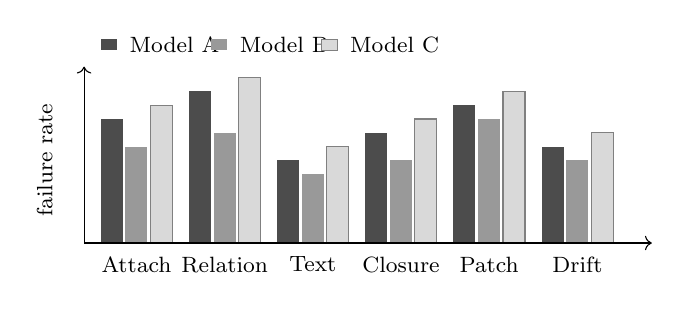
\begin{tikzpicture}[scale=0.7,every node/.style={font=\footnotesize}]
    \def\cats{{"attach","relation","text","closure","patch","drift"}}
    \foreach \v/\name/\a/\b/\c in {
        0/Attach/0.45/0.35/0.50,
        1/Relation/0.55/0.40/0.60,
        2/Text/0.30/0.25/0.35,
        3/Closure/0.40/0.30/0.45,
        4/Patch/0.50/0.45/0.55,
        5/Drift/0.35/0.30/0.40
    } {
      \pgfmathsetmacro{\x}{\v*1.6}
      \fill[black!70] (\x,0) rectangle ++(0.4,\a*5);
      \fill[black!40] (\x+0.45,0) rectangle ++(0.4,\b*5);
      \fill[black!15,draw=black!50] (\x+0.9,0) rectangle ++(0.4,\c*5);
      \node[below=0.05cm] at (\x+0.65,0) {\name};
    }
    \draw[->] (-0.3,0) -- (10,0);
    \draw[->] (-0.3,0) -- (-0.3,3.2);
    \node[rotate=90,anchor=south] at (-0.7,1.5) {failure rate};
    % legend
    \fill[black!70] (0,3.5) rectangle ++(0.3,0.2); \node[anchor=west] at (0.35,3.6) {Model A};
    \fill[black!40] (2,3.5) rectangle ++(0.3,0.2); \node[anchor=west] at (2.35,3.6) {Model B};
    \fill[black!15,draw=black!50] (4,3.5) rectangle ++(0.3,0.2); \node[anchor=west] at (4.35,3.6) {Model C};
  \end{tikzpicture}
  \caption{Illustrative form of the planned headline figure: failure
    rates by category across models. Values shown are placeholders;
    the empirical study is deferred to a follow-up.}
  \label{fig:bar-placeholder}
\end{figure}

% =====================================================================
\section{Related Work}
% =====================================================================

Our framing draws on three strands. \emph{Text-to-image evaluation}
\cite{drawbench,geneval} grades alignment of generated images to
prompts and is the closest neighbour in spirit, although it operates
on pixel synthesis rather than process. \emph{Vector and symbolic
visual representation} \cite{svgenius,vcode} evaluates LLMs on SVG
and related symbolic outputs, and is directly relevant to our claim
that emitting valid markup is not the same as drawing. \emph{Sketch
generation and sketch datasets} \cite{clipdraw,sketchrnn,sketchy}
study sketching as a generative act, often using strokes as the
modelling unit; we adopt the stroke-as-process view but pair it with
agentic repair, which most prior sketch work does not address.

We are gently positioning against a casual claim, common in
practitioner discourse, that LLMs ``can draw'' because they can emit
SVG or Canvas snippets that render to recognisable images. We
believe this confuses fluent emission with reliable construction. We
are building on, not opposing, the body of work that takes drawing
seriously as a structured, evaluable behaviour.

% =====================================================================
\section{Limitations}
% =====================================================================

This paper reports observations from a single production pipeline.
The phenomena we describe are recurrent in that pipeline, but the
empirical study that would let us claim rates of occurrence across
models is deferred. The taxonomy is a working taxonomy and is likely
to evolve; we expect at least one additional named failure to emerge
once the cross-model study is run. Finally, our scope excludes
photorealistic synthesis and 3D; readers working in those areas will
find some claims do not transfer cleanly.

% =====================================================================
\section{Conclusion}
% =====================================================================

A model that can describe a hand is not yet a model that can keep the
wrist attached. We have argued that current LLMs lack a durable
latent canvas: a representation of object identity, part ownership,
contact, and mark history that survives generation and revision.
\inky{}'s working pipeline compensates with external structure ---
construction artifacts, visual feedback, and a strict
\emph{root-cause redraw} rule --- and this compensation works well
enough to ship animations. But the right long-term fix is internal,
not external. Until models can repair drawings the way they repair
code, we should evaluate them as we have proposed: on process,
structure, and repair behaviour, not only on the final image.

% =====================================================================
\section*{Acknowledgements}
% =====================================================================

The author thanks the practitioners and reviewers whose feedback on
the \inky{} pipeline shaped the taxonomy presented here, and the
broader research community working on multimodal evaluation, vector
representations, and sketch generation, whose work this paper builds
on.

% =====================================================================
\begin{thebibliography}{99}
\small
\bibitem{drawbench}
  Saharia, C.\ et al.\ \emph{Photorealistic Text-to-Image Diffusion
  Models with Deep Language Understanding} (Imagen / DrawBench).
  NeurIPS, 2022.

\bibitem{geneval}
  Ghosh, D.\ et al.\ \emph{GenEval: An Object-Focused Framework for
  Evaluating Text-to-Image Alignment.} NeurIPS, 2023.

\bibitem{svgenius}
  \emph{SVGenius: Benchmarking LLMs on Vector Graphics
  Understanding and Generation.} 2024.

\bibitem{vcode}
  \emph{VCode: Code-as-Visual Representation for Language Models.}
  2024.

\bibitem{clipdraw}
  Frans, K., Soros, L.\ B., Witkowski, O.\ \emph{CLIPDraw:
  Exploring Text-to-Drawing Synthesis through Language-Image
  Encoders.} NeurIPS, 2022.

\bibitem{sketchrnn}
  Ha, D., Eck, D.\ \emph{A Neural Representation of Sketch
  Drawings.} ICLR, 2018.

\bibitem{sketchy}
  Sangkloy, P.\ et al.\ \emph{The Sketchy Database: Learning to
  Retrieve Badly Drawn Bunnies.} SIGGRAPH, 2016.

\end{thebibliography}

\onecolumn
\appendix

\section{Failure mode quick reference}
\label{app:quickref}

\begin{table}[h!]
  \small
  \centering
  \begin{tabular}{@{}p{3cm}p{5cm}p{6cm}@{}}
    \toprule
    \textbf{Phenomenon} & \textbf{Signature} & \textbf{Common trigger} \\
    \midrule
    Stroke amnesia & Construction marks become final objects; speech-bubble tail tracks wrong speaker. & Lack of durable mark ownership across the generation loop. \\
    \quad\textit{(inter-frame variant)} & Correct keyframe attachment; broken attachment in the intervening frames. & Sequence-level loss of identity even when single frames are correct. \\
    Compositional collapse & Relational failures rise non-linearly with constraint count. & Multiple simultaneous spatial relations and contacts. \\
    Patch reflex & Defects covered (white plugs, opacity tricks, texture) rather than rebuilt. & Critique phrased as ``fix this'' without anchoring back to construction. \\
    \bottomrule
  \end{tabular}
\end{table}

\section{Prompt suite (preview)}
\label{app:prompts}

The following prompts will be used in the planned empirical study.
Final wording and rendering targets will be frozen at evaluation
time and released with the dataset.

\begin{enumerate}[leftmargin=*,nosep,itemsep=0.3em]
  \item Cat to the left of a kettle on a table.
  \item Person wearing shorts, seated on a chair, both legs visible.
  \item Two characters in conversation, both bubbles visible and correctly owned.
  \item Hand holding a mug by its handle, fingers visible through the handle.
  \item Office scene with five labelled sticky notes.
  \item Ball moving through three frames without rendering guide arrows.
  \item Thought bubble and speech bubble in the same panel, distinguishable.
  \item Plant in pot: rim, soil, stem, leaves, and a water spill.
\end{enumerate}

\section{Reproducibility note}
\label{app:repro}

The \inky{} pipeline described in this paper is implemented in
JavaScript over Canvas 2D, with a node-based tool layer for
rendering and review (Node $\geq$ 22, Vite for the browser
runtime). Reproducibility is at the project level rather than
the example level: from any user-provided storyboard, the
pipeline generates a fresh project scaffold containing
requirements, source lighthouses, construction blueprints,
in-between plans, semantic review boards, visual diffs, and
frame schedules, all in per-project folders. The full set of
pipeline stages is exposed as \texttt{npm run storyboard:*}
commands (\texttt{start}, \texttt{blueprint}, \texttt{inbetween},
\texttt{captions}, \texttt{speech-bubbles}, \texttt{polish},
\texttt{visual-diff}, \texttt{semantic}, \texttt{review},
\texttt{materials}, \texttt{render-frames}). No specific
example projects are preloaded as part of the reproducibility
surface. The companion data release accompanying the planned
empirical study will include the prompt suite, generated code
per model, rendered outputs, and scoring sheets, each produced
through this generic pipeline rather than against a fixed
showcase. The repository, including this paper, is available at
\url{https://github.com/poonamsnair/inky}.

\end{document}
